\documentclass{beamer}
\usetheme{metropolis}
\usepackage[sloppy=false, thaifont=TH Sarabun New]{thaispec}
\usepackage{listings}
\lstset{
  backgroundcolor=\color{black},
  basicstyle=\color{white}\ttfamily,
  keywordstyle=\color{cyan},
  commentstyle=\color{green!60!black},
  stringstyle=\color{orange},
  frame=single,
  rulecolor=\color{white},
  numbers=left,
  numberstyle=\tiny\color{gray},
}

%\usebackgroundtemplate{
  %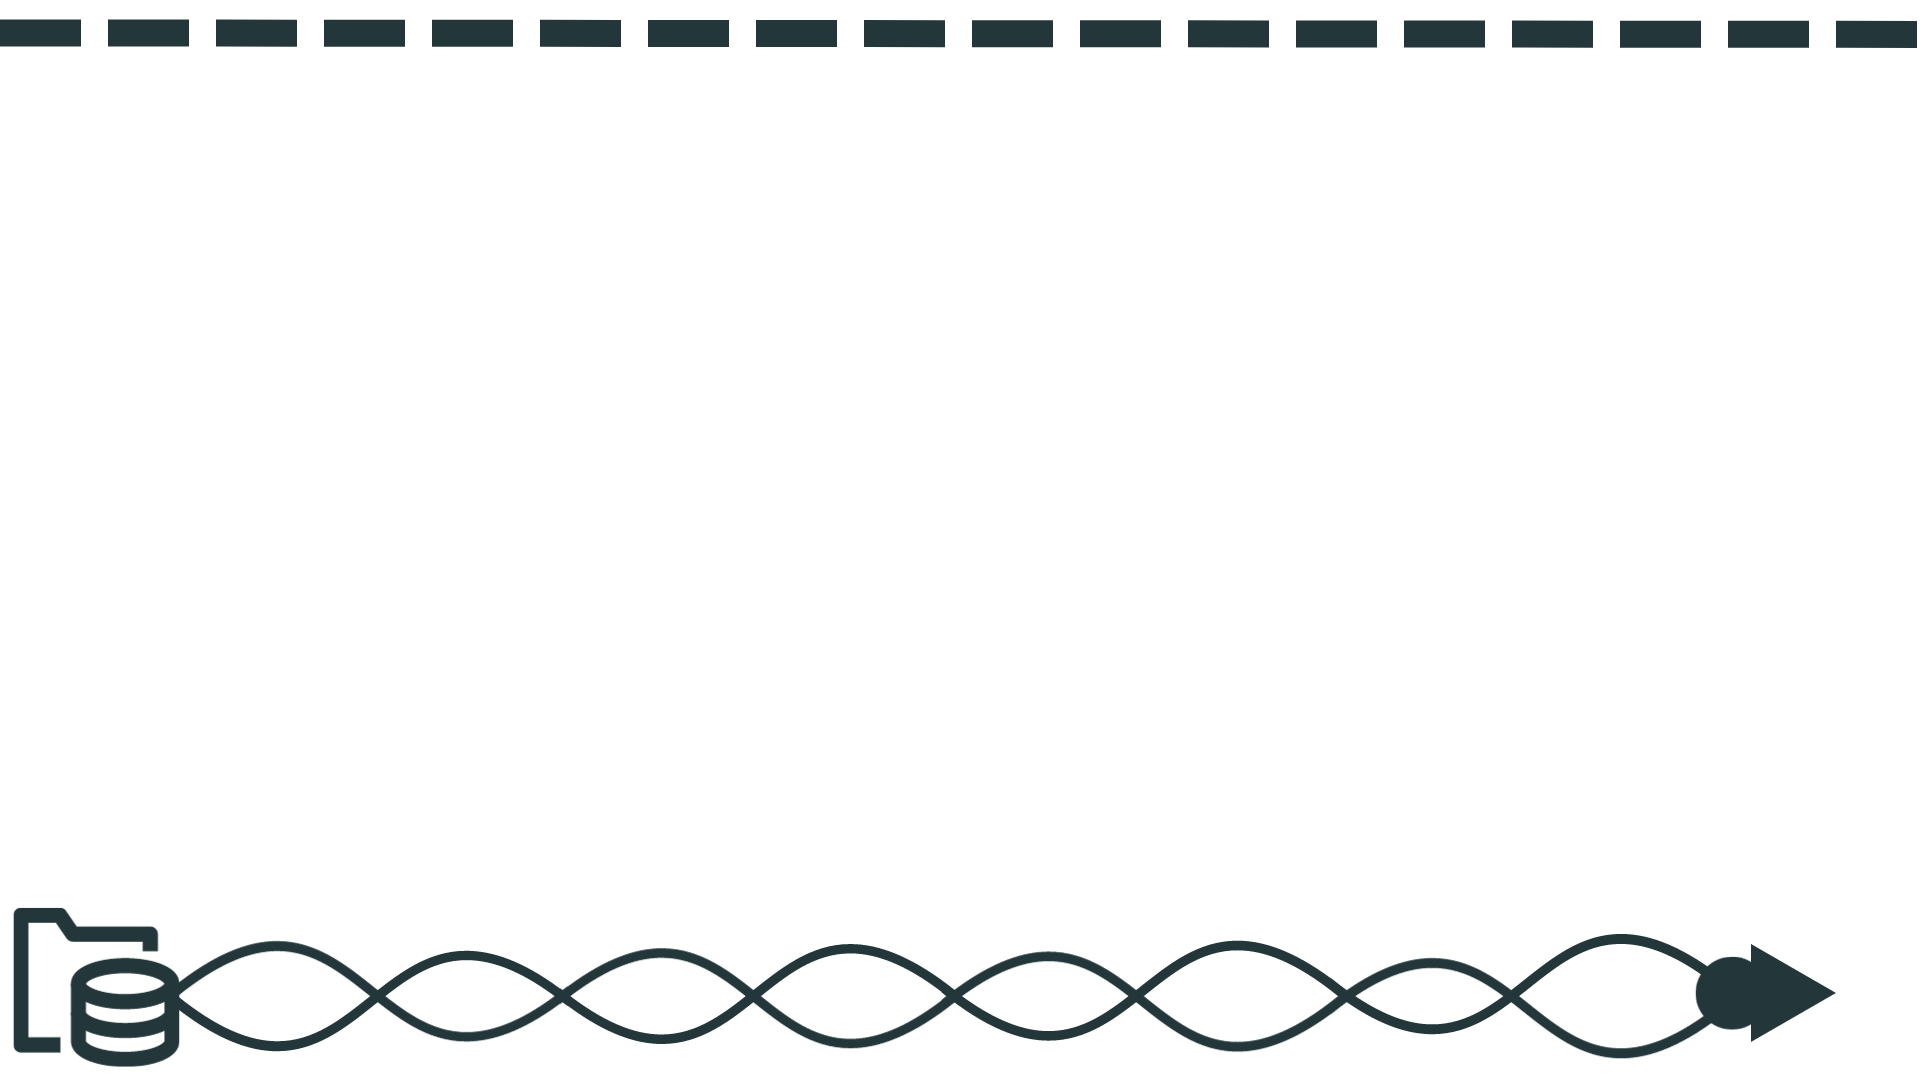
\includegraphics[width=\paperwidth,height=\paperheight]{bg.png}
%}

\title{Database }
\subtitle{กลุ่มผู้เข้าสอบ JLPT}
\date{19 ตุลาคม 2566}
\author{นายณัฐวุฒิ อาจนวลลา 116410901003-6 \\
นายอัฎฐพร จันทร์สุข 116410901011-9 \\
นายคณัสนันท์ ทรัพย์อุดม 116410901033-3 }
\institute{มหาวิทยาลัยเทคโนโลยีราชมงคลธัญบุรี}

\begin{document}

\begin{frame}
  \titlepage
\end{frame}

\begin{frame}{เนื้อหาหลัก}
  \setbeamertemplate{section in toc}[sections numbered]
  \tableofcontents[hideallsubsections]
\end{frame}

\section{ที่มาและความสำคัญ}

\begin{frame}{ที่มาและความสำคัญ}
  \begin{center}
  
\includegraphics[width=0.5\textwidth]{jlpt.png}
  \end{center}
  \vfill
  การจัดสอบ JLPT ถือเป็นอีกหนึ่งการจัดสอบที่สำคัญของประเทศญี่ปุ่น ซึ่งทางการญี่ปุ่นจำเป็นจะต้องออกงบประมาณเพื่อทำการจัดสอบ ดังนั้นกลุ่มเราจึงมีความสนใจที่จะเอาข้อมูลของผู้เข้าสอบของแต่ละประเทศมาวิเคราะห์เพื่อดูแนวโน้มว่าแต่ละประเทศมีความสนใจที่จะเข้าสอบภาษาญี่ปุ่นเป็นอย่างไร และประเทศญี่ปุ่นจะได้กำไรจากการจัดสอบมากแค่ไหน 
\end{frame}

\section{ER Diagram}

\begin{frame}{ER Diagram}
  ข้อมูลในการทำ Database ของกลุ่มเราสามารถแสดงเป็น ER Diagram ได้ดังนี้
  \vfill
  \begin{center}
  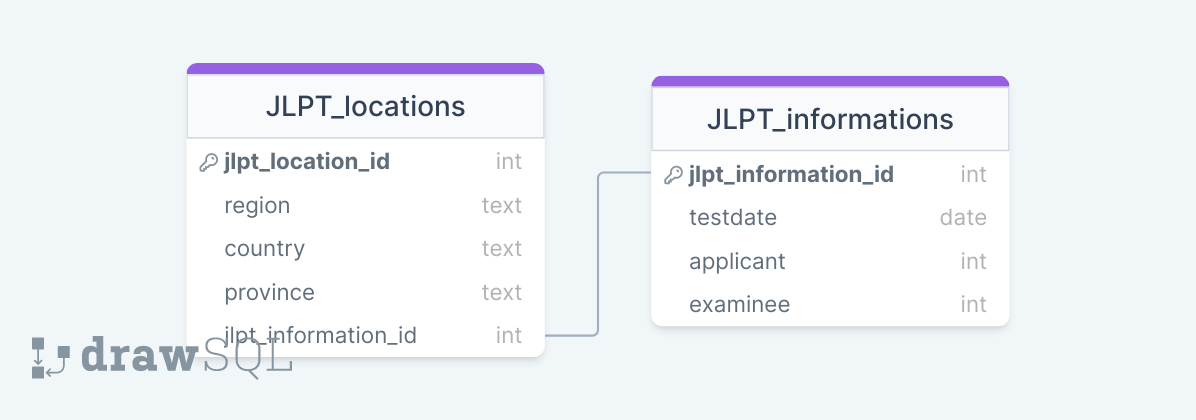
\includegraphics[scale=0.25]{Real_picture.png}
  \end{center} 
\end{frame}

\section{การตั้งคำถาม}

\begin{frame}{การตั้งคำถาม}
  กลุ่มของเราได้ตั้งคำถามขึ้นเพื่อให้ง่ายต่อการค้นหาข้อมูลที่จะใช้ทำ Database ไว้ดังนี้
  \begin{enumerate}
    \item จงเปรียบเทียบผู้เข้าสอบทั้งหมดในวันที่ 2 ม.ค. 2022 กับผู้เข้าสอบทั้งหมดในวันที่ 3 ธ.ค. 2022 
    \item จังหวัดที่มีผู้สมัครสอบมากที่สุดในแต่ละประเทศ 
    \item แสดงประเทศที่มีผู้ใช้สิทธิสอบมากที่สุด 5 อันดับแรก
    \item จงเปรียบเทียบสัดส่วนเปอร์เซ็นต์ผู้เข้าสอบจริงในยุโรป กับ ผู้เข้าสอบจริงในเอเชียตะวันออก
    \item สมมติให้ญี่ปุ่นลงทุนกับการจัดสอบ JLPT 1,000,000,000 เยน ในปี 2022 จงแสดงว่าถ้าญี่ปุ่นจัดสอบในวันที่ 2 ม.ค. 2022 และ 3 ธ.ค. 2022 ญี่ปุ่นจะได้กำไร หรือ ขาดทุนเท่าใด
\end{enumerate}
\end{frame}

\section{คำสั่งในการ Query และผลลัพธ์}

\begin{frame}[fragile]{คำสั่งในการ Query และผลลัพธ์: ข้อที่ 1}
  จงเปรียบเทียบผู้เข้าสอบทั้งหมดในวันที่ 2 ม.ค. 2022 กับผู้เข้าสอบทั้งหมดในวันที่ 3 ธ.ค. 2022
  \begin{lstlisting}[language=SQL]
  SELECT 
      testdate,
      SUM(examinee) AS total_examinees
  FROM JLPT_informations
  GROUP BY testdate;
  \end{lstlisting}
  \begin{table}[ht]
    \centering
    \begin{tabular}{|c|c|}
      \hline
      \textbf{testdate} & \textbf{total\_examinees} \\
      \hline
      2022-01-02 & 354960 \\
      2022-12-03 & 429443 \\
      \hline
    \end{tabular}
  \end{table}
\end{frame}

\begin{frame}[fragile]{คำสั่งในการ Query และผลลัพธ์: ข้อที่ 2}
  จังหวัดที่มีผู้สมัครสอบมากที่สุดในแต่ละประเทศ 
  \begin{tiny}
    \begin{lstlisting}[language=SQL]
    CREATE TABLE Answer_table AS
    SELECT 
      JLPT_locations.country AS 'Country',
      JLPT_locations.province AS 'Province',
      SUM(JLPT_informations.examinee) AS 'Real_examinee'
    FROM JLPT_informations
    INNER JOIN JLPT_locations
    ON JLPT_informations.jlpt_information_id = JLPT_locations.jlpt_information_id
    GROUP BY JLPT_locations.province;

    SELECT 
      Country,
      Province,
      MAX(Real_examinee) AS 'Real_examinee'
    FROM Answer_table
    GROUP BY country;
    \end{lstlisting}
  \end{tiny}
\end{frame}

\begin{frame}[fragile]{คำสั่งในการ Query และผลลัพธ์: ข้อที่ 2}
  \begin{tiny}
  \begin{table}
  \begin{tabular}{|c|c|c|}
  \hline
  \textbf{Country} & \textbf{Province} & \textbf{Real\_examinee} \\
  \hline
  Algeria & Algiers & 36 \\
  Argentina & Buenos Aires & 801 \\
  Armenia & Yerevan & 73 \\
  Australia & Sydney & 306 \\
  Austria & Vienna & 300 \\
  Azerbaijan & Baku & 194 \\
  Bangladesh & Dhaka & 5951 \\
  Belgium & Leuven & 127 \\
  Bhutan & Thimphu & 7 \\
  Bolivia & Santa Cruz & 88 \\
  Bosnia and Herzegovina & Sarajevo & 14 \\
  Brazil & Sao Paulo & 1844 \\
  Brunei & Bandar Seri Begawan & 63 \\
  Bulgaria & Sofia & 356 \\
  Cambodia & Phnom Penh & 1902 \\
  Canada & Toronto & 608 \\
  Chile & Santiago & 357 \\
  China & Hong Kong & 12666 \\
  Colombia & Bogota & 116 \\
  Costa Rica & San Jose & 161 \\
  Czech Republic & Brno & 434 \\
  Denmark & Copenhagen & 102 \\
  Dominican Republic & Santo Domingo & 37 \\
  Ecuador & Quito & 90 \\
  El Salvador & San Salvador & 93 \\
  Finland & Helsinki & 181 \\
  \hline
  \end{tabular}
  \end{table}
  \end{tiny}
\end{frame}

\begin{frame}[fragile]{คำสั่งในการ Query และผลลัพธ์: ข้อที่ 2}
  \begin{tiny}
  \begin{table}
  \begin{tabular}{|c|c|c|}
  \hline
  \textbf{Country} & \textbf{Province} & \textbf{Real\_examinee} \\
  \hline
  France & Paris & 1705 \\
  Georgia & Tbilisi & 121 \\
  Germany & Dusseldorf & 767 \\
  Ghana & Accra & 23 \\
  Greece & Athens & 410 \\
  Hungary & Budapest & 694 \\
  India & Pune & 6237 \\
  Indonesia & Jakarta & 5480 \\
  Ireland & Dublin & 147 \\
  Italy & Roma & 668 \\
  Japan & Tokyo & 76837 \\
  Kazakhstan & Almaty & 243 \\
  Korea & Seoul & 25112 \\
  Kyrgyz Republic & Bishkek & 351 \\
  Laos & Vientiane & 217 \\
  Malaysia & Kuala Lumpur & 3520 \\
  Maldives & Male & 5 \\
  Mexico & Mexico City & 899 \\
  Moldova & Chisinau & 69 \\
  Mongolia & Ulaanbaatar & 1662 \\
  Myanmar & Yangon & 45232 \\
  Nepal & Kathmandu & 3748 \\
  Netherlands & Leiden & 136 \\
  New Zealand & Auckland & 192 \\
  Norway & Kongsvinger & 46 \\
  Pakistan & Islamabad & 516 \\
  \hline
  \end{tabular}
  \end{table}
  \end{tiny}
\end{frame}

\begin{frame}[fragile]{คำสั่งในการ Query และผลลัพธ์: ข้อที่ 2}
  \begin{tiny}
  \begin{table}
  \begin{tabular}{|c|c|c|}
  \hline
  \textbf{Country} & \textbf{Province} & \textbf{Real\_examinee} \\
  \hline
  Papua New Guinea & Port Moresby & 59 \\
  Paraguay & Asuncion & 171 \\
  Peru & Lima & 419 \\
  Philippines & Manila & 4126 \\
  Poland & Warsaw & 1120 \\
  Portugal & Porto & 131 \\
  Romania & Bucharest & 483 \\
  Saudi Arabia & Jeddah & 81 \\
  Serbia & Belgrade & 76 \\
  Singapore & Singapore & 2490 \\
  Slovenia & Ljubljana & 58 \\
  Spain & Madrid & 707 \\
  Sri Lanka & Colombo & 18196 \\
  Switzerland & Zurich & 340 \\
  Taiwan & Taipei & 30802 \\
  Tajikistan & Dushanbe & 68 \\
  Thailand & Bangkok & 17968 \\
  Trinidad and Tobago & Saint Augustine & 13 \\
  Turkey & Ankara & 328 \\
  Turkmenistan & Ashgabat & 130 \\
  U.K. & London & 1000 \\
  U.S.A & Los Angeles & 610 \\
  Uruguay & Montevideo & 134 \\
  Uzbekistan & Tashkent & 758 \\
  Venezuela & Caracas & 150 \\
  Vietnam & Hanoi & 25309 \\
  \hline
  \end{tabular}
  \end{table}
  \end{tiny}
\end{frame}

\begin{frame}[fragile]{คำสั่งในการ Query และผลลัพธ์: ข้อที่ 3}
  แสดงประเทศที่มีผู้ใช้สิทธิสอบมากที่สุด 5 อันดับแรก
  \begin{tiny}
    \begin{lstlisting}[language=SQL]
    SELECT 
      JLPT_locations.country,
      SUM(JLPT_informations.examinee) AS 'All_examinee'
    FROM JLPT_locations
    INNER JOIN JLPT_informations
    ON JLPT_locations.jlpt_information_id = JLPT_informations.jlpt_information_id
    GROUP BY JLPT_locations.country
    ORDER BY SUM(JLPT_informations.examinee) DESC
    LIMIT 5;
    \end{lstlisting}
  \end{tiny}
  \begin{table}[ht]
  \centering
    \begin{tabular}{|c|c|}
      \hline
      \textbf{Country} & \textbf{All\_examinee} \\
      \hline
      Japan & 331303 \\
      China & 77924 \\
      Taiwan & 66419 \\
      Myanmar & 57888 \\
      Korea & 57172 \\
      \hline
    \end{tabular}
  \end{table}
\end{frame}

\begin{frame}[fragile]{คำสั่งในการ Query และผลลัพธ์: ข้อที่ 4}
  จงเปรียบเทียบสัดส่วนเปอร์เซ็นต์ผู้เข้าสอบจริงในยุโรป กับ ผู้เข้าสอบจริงในเอเชียตะวันออก
  \begin{tiny}
    \begin{lstlisting}[language=SQL]
    SELECT 
      JLPT_locations.region AS 'Region',
      CAST(SUM(JLPT_informations.examinee) AS REAL)/
      CAST(SUM(JLPT_informations.applicant) AS REAL)*100 
      AS 'Examinee(%)'
    FROM JLPT_informations
    INNER JOIN JLPT_locations
    ON JLPT_informations.jlpt_information_id = JLPT_locations.jlpt_information_id
    WHERE Region = 'Europe' OR Region = 'East Asia'
    GROUP BY JLPT_locations.region;
    \end{lstlisting}
  \end{tiny}
  \begin{table}[ht]
  \centering
    \begin{tabular}{|c|c|}
      \hline
      \textbf{Region} & \textbf{Examinee(\%)} \\
      \hline
      East Asia & 85.8458657484438 \\
      Europe & 86.607617360496 \\
      \hline
    \end{tabular}
  \end{table}
\end{frame}

\begin{frame}[fragile]{คำสั่งในการ Query และผลลัพธ์: ข้อที่ 5}
  สมมติให้ญี่ปุ่นลงทุนกับการจัดสอบ JLPT 1,000,000,000 เยน ในปี 2022 จงแสดงว่าถ้าญี่ปุ่นจัดสอบในวันที่ 2 ม.ค. 2022 และ 3 ธ.ค. 2022 ญี่ปุ่นจะได้กำไร หรือ ขาดทุนเท่าใด
  \begin{tiny}
    \begin{lstlisting}[language=SQL]
    SELECT 
      SUM(JLPT_informations.applicant) * 50 AS 'Applicants payment in Japan(USD)',
      6718489.00 AS 'Japan Goverment investment(USD)',
      CASE 
          WHEN (SUM(applicant)*50 - 6718489.00 ) > 0 THEN 'Gain a profit' 
          ELSE 'Loss' 
      END AS Answer
    FROM JLPT_informations
    INNER JOIN JLPT_locations
    ON JLPT_locations.jlpt_information_id = JLPT_informations.jlpt_information_id
    WHERE JLPT_locations.country = 'Japan';
    \end{lstlisting}
  \end{tiny}
  \begin{tiny}
  \begin{table}[ht]
  \centering
    \begin{tabular}{|c|c|c|}
      \hline
      \textbf{Applicants payment in Japan(USD)} & \textbf{Japan Goverment investment(USD)} & \textbf{Answer} \\
      \hline
      18570950 & 6718489.0 & Gain a profit \\
      \hline
    \end{tabular}
  \end{table}
  \end{tiny}
\end{frame}
\end{document}
